% Weight-Space Programming: An Independent Field Guide (whitepaper)
% Compile: tectonic main.tex  (or: python3 $PDF_SKILL_DIR/scripts/pdf.py convert.latex main.tex --runs 2)
% Author of this explainer: Het Patel (Hunterdii). Based on the MIT CSAIL blog post of 2 Nov 2026 (see Credits).
\documentclass[11pt,a4paper]{article}

\usepackage{graphicx}
\usepackage{xcolor}
\usepackage{geometry}
\usepackage{amsmath,amssymb}
\usepackage{booktabs}
\usepackage{longtable}
\usepackage{tabularx}
\usepackage{adjustbox}
\usepackage{listings}
\usepackage[most]{tcolorbox}
\usepackage{enumitem}
\usepackage{titlesec}
\usepackage{fancyhdr}
\usepackage{microtype}
\usepackage[section]{placeins}
\usepackage[numbers,sort&compress]{natbib}
\bibliographystyle{unsrtnat}

% hyperref ALWAYS last among content packages
\usepackage[
  colorlinks=true,
  linkcolor=wspblue,
  citecolor=darkgray,
  urlcolor=wspblue,
  bookmarks=true,
  bookmarksnumbered=true,
  unicode=true
]{hyperref}

\geometry{a4paper, top=2.4cm, bottom=2.4cm, left=2.4cm, right=2.4cm}
\setlength{\headheight}{14pt}
\setlength{\parskip}{0.35em}
\setlength{\parindent}{0em}
\widowpenalty=10000
\clubpenalty=10000
\emergencystretch=1.5em

% ---------- truth-contract palette ----------
\definecolor{wspblue}{HTML}{2F6FD0}   % paper-reported
\definecolor{wspgreen}{HTML}{0E8A5F}  % independent review
\definecolor{wspamber}{HTML}{B57A00}  % teaching schematic
\definecolor{wspred}{HTML}{C03A2F}    % speculation
\definecolor{wspviolet}{HTML}{6D55C8}
\definecolor{inkink}{HTML}{1A1D26}
\definecolor{mutedmut}{HTML}{5D6372}
\definecolor{paperpaper}{HTML}{FAF9F5}

% ---------- badge commands (colour AND text - never colour alone) ----------
\newcommand{\bP}{\textcolor{wspblue}{\rule[0.12ex]{1.5mm}{1.5mm}}\;\textcolor{wspblue}{\textbf{PAPER-REPORTED}}}
\newcommand{\bR}{\textcolor{wspgreen}{\rule[0.12ex]{1.5mm}{1.5mm}}\;\textcolor{wspgreen}{\textbf{INDEPENDENT\,REVIEW}}}
\newcommand{\bS}{\textcolor{wspamber}{\rule[0.12ex]{1.5mm}{1.5mm}}\;\textcolor{wspamber}{\textbf{TEACHING\,SCHEMATIC}}}
\newcommand{\bX}{\textcolor{wspred}{\rule[0.12ex]{1.5mm}{1.5mm}}\;\textcolor{wspred}{\textbf{SPECULATION}}}

\newtcolorbox{plainbox}[1][]{colback=paperpaper, colframe=inkink!22, boxrule=0.6pt, arc=2pt,
  left=6pt, right=6pt, top=5pt, bottom=5pt, #1}
\newtcolorbox{truebox}[1][]{colback=paperpaper, colframe=wspblue!55, boxrule=0.8pt, arc=2pt,
  left=6pt, right=6pt, top=5pt, bottom=5pt, title={\bP}, #1}
\newtcolorbox{onepage}[1][]{colback=paperpaper, colframe=wspviolet!60, boxrule=1.1pt, arc=3pt,
  left=8pt, right=8pt, top=7pt, bottom=7pt, #1}

\lstset{
  basicstyle=\ttfamily\footnotesize,
  breaklines=true,
  frame=single,
  framesep=4pt,
  rulecolor=\color{inkink!25},
  backgroundcolor=\color{paperpaper},
  aboveskip=0.9em,
  belowskip=0.9em,
  language=Python,
  showstringspaces=false,
  xleftmargin=6pt, xrightmargin=6pt,
}

\titleformat{\section}{\Large\bfseries\color{inkink}}{\thesection}{0.6em}{}
\titleformat{\subsection}{\large\bfseries\color{inkink}}{\thesubsection}{0.6em}{}
\titlespacing*{\section}{0pt}{16pt plus 4pt minus 2pt}{8pt plus 2pt minus 1pt}
\titlespacing*{\subsection}{0pt}{12pt plus 3pt minus 2pt}{5pt plus 1pt minus 1pt}

\pagestyle{fancy}
\fancyhf{}
\fancyhead[L]{\footnotesize\color{mutedmut}Weight-Space Programming: An Independent Field Guide}
\fancyfoot[C]{\footnotesize\color{mutedmut}\thepage}
\renewcommand{\headrulewidth}{0.4pt}
\renewcommand{\headrule}{\color{inkink!15}\hrule width\headwidth height\headrulewidth}

\hypersetup{
  pdftitle={Weight-Space Programming: An Independent Field Guide},
  pdfauthor={Het Patel (Hunterdii)},
  pdfsubject={An independent, badge-honest explainer of Weight-Space Programming (WSP): LLMs reading, fixing, and writing neural-network weights by reasoning},
  pdfkeywords={weight-space programming, model editing, interpretability, LLM, neural network weights, benchmarks},
  pdfcreator={LaTeX via Tectonic}
}

\begin{document}

% ════════════════════════════ TOC (first body page; cover is merged in front) ════════════════════════════
{\hypersetup{linkcolor=inkink}\tableofcontents}
\newpage

% ════════════════════════════ IF YOU READ ONE PAGE ════════════════════════════
\begin{onepage}
{\color{wspviolet}\bfseries IF YOU READ ONE PAGE}\par\vspace{3pt}
\textbf{The finding.} A blog post from MIT CSAIL (2~Nov~2026) reports that a general-purpose LLM can \emph{read} a small neural network's weights and say what it does, \emph{fix} a defect with one reasoned edit, and even \emph{write} working networks from scratch --- all without gradient descent \cite{wsp-post}.

\textbf{The headline number.} Editing \textbf{0.016\%} of a small math model's weights (131{,}072 of ${\sim}0.8$B) raised MATH-500 from 7.9\% to 48.1\%, cut runaway ``thinking'' from 93\% to 33\% of answers --- and a \emph{negative control} on a different model moved nothing, showing the edit removed an obstacle rather than conjuring ability \cite{wsp-post}.

\textbf{The honest caveats.} Every result is a single run; baselines (decoding tweaks, textbook direction-ablation, ordinary code) are missing; tasks were designed by the authors. An independent review sorts the evidence from strong (the math fix) to anecdotal (small reading games) \cite{maier}, and a second essay argues the deflationary case across all eight experiments \cite{goedecke}.

\textbf{This document} is an independent explainer: it rebuilds the whole topic from zero, badges every claim by evidence class, ships runnable labs, and proposes the benchmark the evidence is waiting for.
\end{onepage}

\vspace{0.8em}
\begin{abstract}
\noindent Weight-Space Programming (WSP) is the claim that a general-purpose large language model can read a neural network's parameters, diagnose them, and modify them --- or synthesise them from scratch --- through reasoning alone, optionally verified by a handful of forward passes. This whitepaper is an independent educational treatment of the finding, built around a strict evidential discipline: every figure, number, and claim carries exactly one of four badges (paper-reported, independent review, teaching schematic, speculation). We condense the original post's eight experiments, reconstruct their mechanisms with worked mathematics and three runnable labs, weigh them against the two published third-party assessments, and map both the authors' five predictions and a fuller horizon of futures and risks. We contribute WSP-Bench-Lite, a community benchmark proposal (Read/Fix/Write tracks, author-blind tasks, mandatory baselines, $\geq$5 seeds, drift and sparsity metrics) designed to close the specific evidential gaps the independent reviews identified. The reader journey runs from ``what is a weight?'' to ``how would I design the next experiment?''
\end{abstract}

\section*{How to read this document}
\addcontentsline{toc}{section}{How to read this document}

This whitepaper is badged, and the badges are load-bearing. Every figure, number, and sentence-level claim carries \emph{exactly one} of four evidence markers, in colour \emph{and} text (never colour alone):

\begin{itemize}[leftmargin=1.8em, itemsep=2pt]
\item \bP\; --- a number or claim stated in the original post (2~Nov~2026). Transcribed, not independently re-measured.
\item \bR\; --- from a third-party analysis (principally the 5~Nov~2026 review).
\item \bS\; --- made-up toy data created by this guide to explain an idea. Illustrative, not real data; figures are marked in their captions.
\item \bX\; --- speculation about the future, including the original authors' own, untested.
\end{itemize}

Three reading paths. \emph{The fifteen-minute path:} the one-page box above, Figure~\ref{fig:scoreboard}, and the conclusion. \emph{The practitioner path:} Sections~\ref{sec:fourways}--\ref{sec:mech} for the experiments and mechanisms, Appendix~D for the runnable labs, and Appendix~E for the benchmark schema. \emph{The reviewer path:} Sections~\ref{sec:judgement}--\ref{sec:lab} in full, then Appendix~C (open verification items) --- which is the part of this document most likely to change first.

\vspace{0.5em}
\begin{plainbox}[title={\bfseries Credits and non-affiliation}]
\small
\textbf{Independent educational explainer by Het Patel (Hunterdii)}, MSc Data Science student. Based on the blog post \emph{``Sparks of Weight-Space Programming: LLMs can natively read \& write neural network weights''} by Rikiya Takehi, Jayden Teoh, Alex Zhang and Omar Khattab (MIT CSAIL), 2~Nov~2026. All original research credit belongs to them. This project is \textbf{not affiliated with, endorsed by, or written by} MIT CSAIL, OpenAI, or the original authors. Items labelled \emph{Het's Lab} are independent additions, clearly marked. Licence: code MIT, text \& figures CC~BY~4.0. Cite the original post when citing results. Fact-check date: 5~Nov~2026; unresolved items are listed in Appendix~C.
\end{plainbox}

\section{A Network Is a Pile of Numbers}\label{sec:pile}

Every neural network --- game player, chat model, image maker --- is fully described by a long list of real numbers. Formally, a network is a function $f_\theta(x)$ whose behaviour is fixed by a parameter vector
\begin{equation}\label{eq:network}
\theta \in \mathbb{R}^{P}, \qquad P = \sum_{i}\bigl(d_i d_{i+1} + d_{i+1}\bigr)
\end{equation}
for a stack of layers with widths $d_0 \to d_1 \to \dots$. The wiring is the \emph{architecture} --- an MLP here, a transformer \cite{attention} elsewhere, a vision transformer \cite{vit} for images --- and the numbers filling it are the \emph{weights}. The single most important sentence in this document is: \textbf{same architecture + different numbers = different skill}. Two piles of 17{,}253 numbers with identical wiring can differ as much as a Breakout player differs from a Pong player --- which is precisely the warm-up experiment of the source post \cite{wsp-post}.

\bP\; In Experiment~1, the reader model saw a $10\times10$ grid of first-layer weights from a $500{\to}32{\to}32{\to}5$ tanh MLP (P~$=$~17{,}253, consistent with Eq.~\eqref{eq:network}) trained with PPO on one of four Atari-like games, and named all four correctly --- Breakout at 99\% stated confidence, with no forward passes allowed.

\begin{figure}[htbp]
\centering
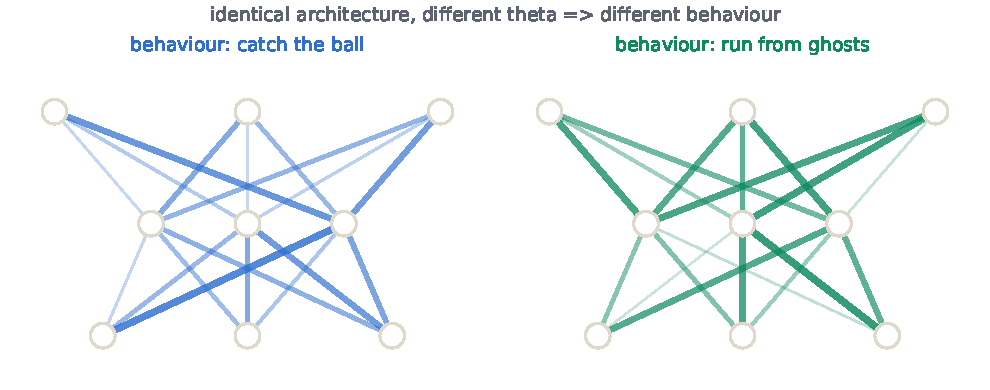
\includegraphics[width=0.86\linewidth]{figures/fig01_anatomy.pdf}
\caption{\bS\; Two networks with identical wiring but different $\theta$ compute different behaviours. Illustrative, not real data.}
\label{fig:anatomy}
\end{figure}

\bS\; The natural mental image is a \emph{landscape}: define a loss $L(\theta)$ and weight space becomes a high-dimensional surface on which training is a long walk (Figures~\ref{fig:anatomy} and \ref{fig:landscape}). A crucial subtlety undercuts naive reading: many different $\theta$ compute the \emph{same} function, because permuting hidden units changes every weight without changing behaviour. Reading behaviour from weights is therefore underdetermined up to symmetries --- a structure well studied in the lottery-ticket and re-basin lineages \cite{lottery,gitrebasin} --- so the reader must find invariants, a theme that explains much of Section~\ref{sec:read}.

\begin{figure}[htbp]
\centering
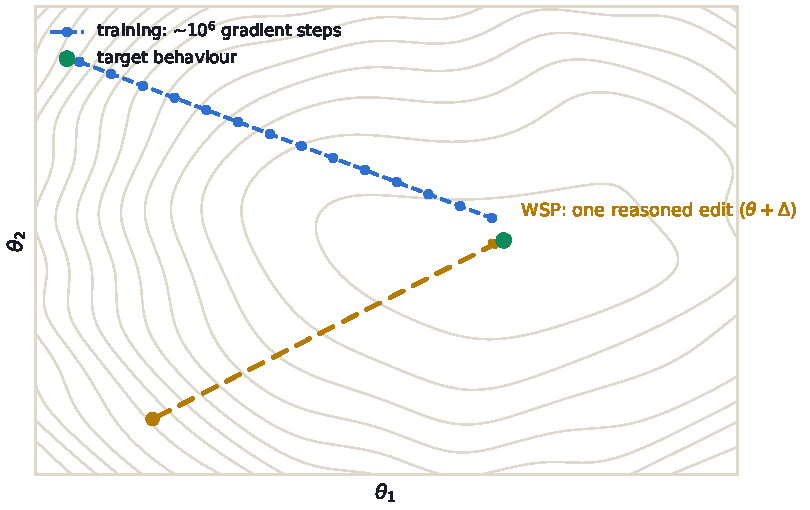
\includegraphics[width=0.72\linewidth]{figures/fig02_landscape.pdf}
\caption{\bS\; Weight space as a loss landscape: training walks ($\sim$$10^6$ gradient steps); a weight-space edit is one reasoned jump. Illustrative, not real data.}
\label{fig:landscape}
\end{figure}

\section{Four Ways to Write Weights}\label{sec:fourways}

Before November 2026, parameters were written in three ways. \textbf{(1) Optimisation.} Gradient descent and its descendants (SGD, Adam, Muon) take millions of tiny steps:
\begin{equation}\label{eq:sgd}
\theta_{t+1} = \theta_t - \eta\,\nabla_\theta \mathcal{L}(\theta_t),
\end{equation}
consuming datasets and compute at industrial scale \cite{adam,muon} --- the way every frontier language model to date was trained \cite{gpt3} --- and the PPO baselines of the post consumed $10^8$--$10^9$ environment steps \cite{ppo}. \textbf{(2) Trained writers.} Hypernetworks $g_\phi(z)\!\to\!\theta$ output other networks' weights \cite{ha}; fast-weight programmers write temporary weights at run time \cite{schlag}; diffusion over weights generates parameter sets from learned distributions \cite{nndiffusion}. All require a corpus of training networks first. \textbf{(3) Compilers.} Tracr compiles a formal RASP program directly into transformer weights, interpretable by construction \cite{tracr} --- but only for hand-written, toy-scale programs.

\bP\; The post proposes a fourth way:
\begin{equation}\label{eq:wsp}
\theta' = \theta + \Delta, \qquad \Delta = \mathrm{LLM}\bigl(\theta,\ \text{spec},\ \text{optional feedback}\bigr),
\end{equation}
where the writer is a general-purpose LLM never trained to write weights, the edit is conditioned on the actual current $\theta$, and a handful of forward passes may serve as feedback. The claimed discontinuity is \emph{understanding-first writing}: the edit arrives with a readable reasoning trace.

\begin{figure}[htbp]
\centering
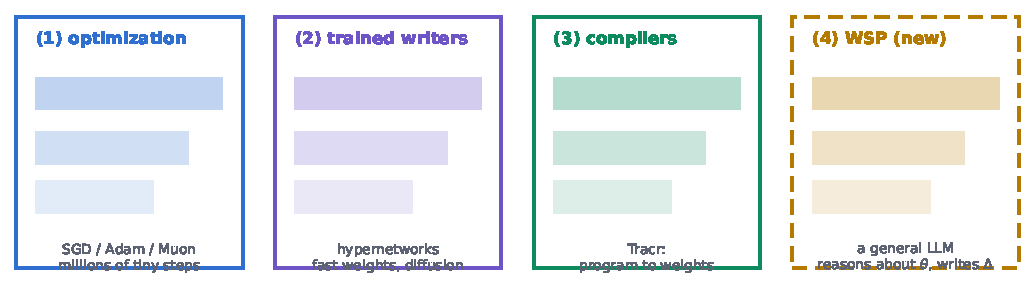
\includegraphics[width=0.98\linewidth]{figures/fig03_fourways.pdf}
\caption{\bS\; The four ways weights get written. Ways (1)--(3) predate the post; way (4) is its claim. Illustrative.}
\label{fig:fourways}
\end{figure}

\bP\; The cost asymmetry, in the post's own numbers: PPO needed $10^8$--$5{\times}10^8$ environment steps to reach 15.8--25.3 on MinAtar Breakout, while the written policy reached 517.4 in one shot with zero environment steps --- and up to 50 forward passes for the Go policy. Even granting that these are different task families, the compute gap spans six orders of magnitude. Against that stands a context-window reality check: weights must \emph{reach} the reasoner. Experiment~3 fed 7.16M parameters (middle blocks only); the flagship edit worked on two selected MLP blocks rather than the whole 0.8B. So ``an LLM reads the model'' is, in practice, ``an LLM reads surgical slices plus summary statistics'' --- and any production WSP needs slicing, aggregation, and selective read-out tooling, which is what the released logs effectively hand-rolled.

\bR\; The review's sharpest standing question \cite{maier}: for each reported edit, could a \emph{cheap standard alternative} --- a decoding change, a textbook direction ablation, or the same heuristic as ordinary code --- achieve the same effect? Until that is answered, ``WSP works'' must not be confused with ``WSP is the right tool.''

\section{Cousins: Who Else Touches the Weights?}\label{sec:cousins}

WSP joins a crowded family. Fine-tuning re-runs the loop of Eq.~\eqref{eq:sgd} on new data. LoRA constrains the change to a low-rank cone,
\begin{equation}\label{eq:lora}
W' = W + \tfrac{\alpha}{r}BA, \qquad B \in \mathbb{R}^{d\times r},\ A \in \mathbb{R}^{r\times k},
\end{equation}
training ${\sim}0.5\%$ as many numbers \cite{lora}. Task arithmetic moves along lines between checkpoints \cite{ilharco},
\begin{equation}\label{eq:taskarith}
\theta_{\text{new}} = \theta_{\text{base}} + \lambda \tau, \qquad \tau = \theta_{\text{ft}} - \theta_{\text{base}},
\end{equation}
and merging blends several such models \cite{ties}. Model editing solves a closed-form rank-one update for one fact \cite{rome},
\begin{equation}\label{eq:rome}
\Delta W = \frac{(v^{*} - Wk^{*})(C^{-1}k^{*})^{\top}}{(C^{-1}k^{*})^{\top} k^{*}}.
\end{equation}
Activation steering bends behaviour at run time with weights frozen; mechanistic interpretability reads circuits without writing \cite{elhage,olsson,nanda}; the weight-space-learning survey and its companion repo frame the field's three branches of understanding, representation, and generation \cite{wslsurvey,awesomewsl}. Table~\ref{tab:cousins} sorts the family along the axes that matter.

\begin{table}[htbp]
\centering
\small
\caption{\bS\; Who writes the weights? A teaching summary --- qualitative ratings for orientation, not measured comparisons.}
\label{tab:cousins}
\begin{tabularx}{\linewidth}{l >{\raggedright\arraybackslash}X l l l}
\toprule
Method & Mechanism & Data & Gradients & Diff readable? \\
\midrule
Training / fine-tuning & follow $\nabla\mathcal{L}$ (Eq.~\ref{eq:sgd}) & heavy & yes & no \\
LoRA (Eq.~\ref{eq:lora}) & low-rank $\Delta$, still gradients & task set & yes & partly \\
Task arithmetic (Eq.~\ref{eq:taskarith}) & add/subtract checkpoints & 2 models & no & vector \\
Model editing (Eq.~\ref{eq:rome}) & closed-form, one fact & one pair & no & yes (rank-1) \\
Activation steering & runtime add $\alpha u$ & a direction & no & vector (runtime) \\
Mech.\ interpretability & reverse-engineer circuits & --- & no & --- (read-only) \\
Tracr compile & program $\to$ weights & formal spec & no & yes \\
WSP (Eq.~\ref{eq:wsp}) & reason about $\theta$, write $\Delta$ & a spec & no & reasoned trace \\
\bottomrule
\end{tabularx}
\end{table}

\bP\; One cousin deserves special mention for what it implies about risk (Section~\ref{sec:risks}): published work shows that \emph{refusal} in open models is mediated by a single direction, removable by projection \cite{refusal} --- the same mathematical operation class the flagship fix uses (Eq.~\ref{eq:direction} below).

\section{READ: Guessing Games with Real Weight Lists}\label{sec:read}

Four experiments test the reading claim. \bP\; Exp.~1 (games): four PPO-trained MLP policies (Breakout, Pong, Pac-Man, Freeway), each 17{,}253 parameters, presented as $10{\times}10$ first-layer grids, no tools; the reader named all four games, Breakout at 99\% confidence. Exp.~2 (shapes): three 23{,}824-parameter DDPM \cite{ddpm} noise-predictors generating $12{\times}12$ circle/triangle/square images; all three identified without a forward pass --- but described as \emph{outlines} while the models draw \emph{filled} shapes: a correct yet lossy read. Exp.~3 (languages): three char-level transformers ($4$ layers $\times$ $6$ heads, width 384, 7.16M parameters), middle blocks only, running banned; language identified in 6/6 attempts at 0.48--0.62 confidence, and \emph{copying heads exactly matched measured ground truth}: Python 2.1, 3.1, 3.5; romaji 3.3; English 3.1. Exp.~7 (sycophancy): two Gemma-3-270M \cite{gemma3} twins fine-tuned identically except the answer rule; weights alone failed 0/4, but with attention patterns on self-written texts the honest/sycophantic pair was identified 3/3.

\begin{table}[htbp]
\centering
\small
\caption{\bP\; The READ experiments at a glance (all values from the post).}
\label{tab:read}
\begin{tabularx}{\linewidth}{c >{\raggedright\arraybackslash}X l >{\raggedright\arraybackslash}X}
\toprule
\# & Task & Weights shown & Reported result \\
\midrule
1 & which game? & 17{,}253 (grid) & 4/4 named; Breakout 99\% \\
2 & which shape (DDPM)? & 23{,}824 & 3/3 correct; outlines vs filled \\
3 & which language + which heads copy? & 7.16M (middle blocks) & 6/6 language (conf.\ 0.48--0.62); heads exact \\
7 & which Gemma flatters? & ${\sim}$270M $\times$ 2 & weights alone 0/4; with activations 3/3 \\
\bottomrule
\end{tabularx}
\end{table}

\begin{figure}[htbp]
\centering
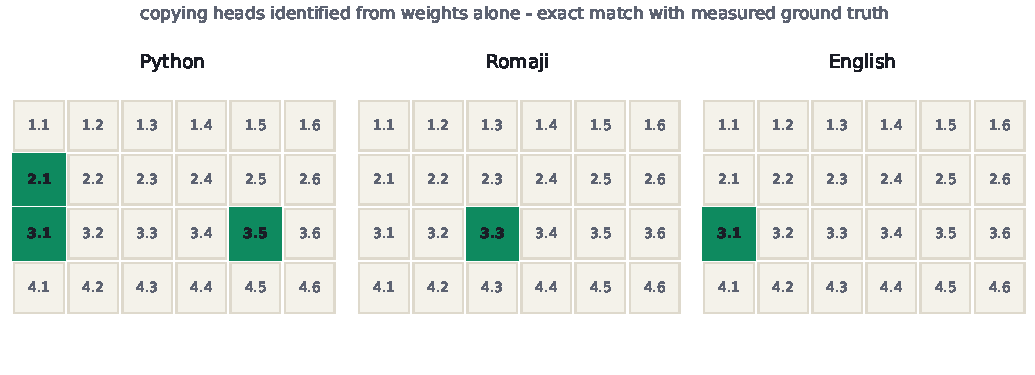
\includegraphics[width=0.95\linewidth]{figures/fig04_headgrid.pdf}
\caption{\bP\; Exp.~3: copying heads identified from weights alone (green), an exact match with the heads measured by running the models --- the solid part of the READ evidence.}
\label{fig:headgrid}
\end{figure}

Why are copying heads findable from static weights? The induction circuit is a two-head composition: head~1 moves the previous token forward; head~2 attends from the later occurrence back and copies what followed. Its signature lives in the product of the two heads' circuits, summarised by the composition score of Elhage et al.~\cite{elhage}:
\begin{equation}\label{eq:induction}
\mathrm{score} = \frac{\bigl\lVert W^{(2)}_{QK} W^{(1)}_{OV} \bigr\rVert_F}{\bigl\lVert W^{(2)}_{QK} \bigr\rVert_F \, \bigl\lVert W^{(1)}_{OV} \bigr\rVert_F}.
\end{equation}
Because Eq.~\eqref{eq:induction} is invariant to head permutations, it survives exactly the symmetries (Section~\ref{sec:pile}) that defeat naive coordinate-by-coordinate reading. The reader model executed this known human technique on raw middle-block weights --- the technique, not a novel capability, is what the exact match certifies.

\bP\; Exp.~7's tell, quantified: on self-written texts, head 10.2 of the honest model places 94.3\% of its attention on the question's numbers versus 0.75\% on the user's answer; the sycophant flips to 3.5\% versus 85.7\% (Figure~\ref{fig:head102}). The signature lives in activations, not weights --- which is the honest limit of that experiment.

\begin{figure}[htbp]
\centering
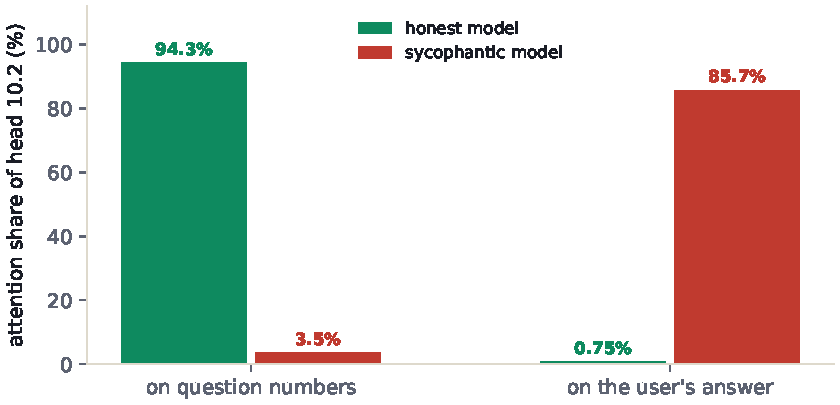
\includegraphics[width=0.68\linewidth]{figures/fig05_head102.pdf}
\caption{\bP\; Exp.~7, head 10.2 attention shares on self-written texts (values from the post).}
\label{fig:head102}
\end{figure}

\bS\; Where could each read ``cheat''? Protocol details matter here, because each experiment was engineered to make reading a genuine test: Experiment~1 banned tools and forward passes (so no behavioural probing), Experiment~3 showed only middle blocks (cutting the easy surface statistics of embedding and output layers), and Experiment~7 froze embeddings and the output layer (so the twins differ only in the rule, not the vocabulary). Against those constraints, three leakage paths remain worth naming: PPO on these four games leaves characteristic first-layer profiles, so strong Atari priors from pre-training could carry Exp.~1; the outline-versus-filled slip in Exp.~2 shows the reader found boundary geometry and missed the fill regime; and Exp.~7 succeeded only after the task was relaxed to weights-plus-activations, which is a different (and weaker) claim than weights alone.

\bR\; The review's sort \cite{maier}: Exps.~1--2 are correct but tiny trials on deliberately readable layouts; the language identification is barely above the 1/3 chance floor; three binary picks (Exp.~7) admit a 1-in-8 lucky run --- and the task had to be relaxed to weights-plus-activations before it worked. The copying-head match is the one solid READ result. Read everything else with those priors.

\section{FIX: Surgery on a Ramp and on a Thought Loop}\label{sec:fix}

\bP\; Exp.~4 (ramp): a Kinetix actor \cite{kinetix} ($679{\to}128{\to}5{\times}128{\to}16$, 171{,}664 parameters) trained with PPO failed a ramp task 256/256 times. One edit, no tools, touching 3.5\% of the actor's weights, flipped success to 1{,}024/1{,}024 episodes. Exp.~8 (math): Qwen3.5-0.8B \cite{qwen3} in thinking mode (up to 32{,}768 tokens) hit the token limit on 93\% of MATH-500 \cite{math500} problems, scoring 7.9\%. The reader identified a \emph{looping direction} written by the MLPs of layers 15 and 19 and subtracted it from the 64 highest-contribution output columns of each layer: 131{,}072 weights, 0.016\% of the model. With 50 feedback passes, MATH-500 reached 48.1\%, GSM8K \cite{gsm8k} 67.1\% (from 13.8\%), IFEval \cite{ifeval} 62.3\% (from 21.0\%), and token-limit hits fell to 33.1\% (Table~\ref{tab:budget}).

\begin{table}[htbp]
\centering
\small
\caption{\bP\; Exp.~8 budget table: Qwen3.5-0.8B, thinking on, up to 32{,}768 tokens.}
\label{tab:budget}
\begin{tabular*}{\linewidth}{@{\extracolsep{\fill}} l cccc}
\toprule
Variant & MATH-500 \% & GSM8K \% & IFEval \% & Token limit \% \\
\midrule
Base & 7.9 & 13.8 & 21.0 & 93.0 \\
Edited, 10 passes & 12.3 & 25.7 & 49.0 & 87.2 \\
Edited, 25 passes & 14.1 & 25.1 & 39.9 & 86.4 \\
Edited, 50 passes & \textbf{48.1} & \textbf{67.1} & \textbf{62.3} & \textbf{33.1} \\
\bottomrule
\end{tabular*}
\end{table}

The mechanism is textbook single-direction surgery \cite{refusal}: compute the projection that zeroes a direction $u$ from selected columns $S$,
\begin{equation}\label{eq:direction}
W' = (I - u u^{\top}) W \ \ \text{on } S, \qquad \Delta = -\,u\,(u^{\top} W)\big|_S, \qquad u^{\top} W' \approx 0,
\end{equation}
shown here in its teaching approximation; the post's exact per-column update lives in its released logs \cite{wsp-logs}. The blast radius of the edit is its sparsity,
\begin{equation}\label{eq:sparsity}
s = \frac{\lVert \Delta \rVert_0}{P} = \frac{131{,}072}{0.8 \times 10^{9}} \approx 1.6 \times 10^{-4} = 0.016\%,
\end{equation}
with the hidden size of 1024 behind the $2 \times 64 \times$ width arithmetic flagged for verification (Appendix~C). Figure~\ref{fig:anatomyedit} sketches where the edit lives inside the 24 layers.

\begin{figure}[htbp]
\centering
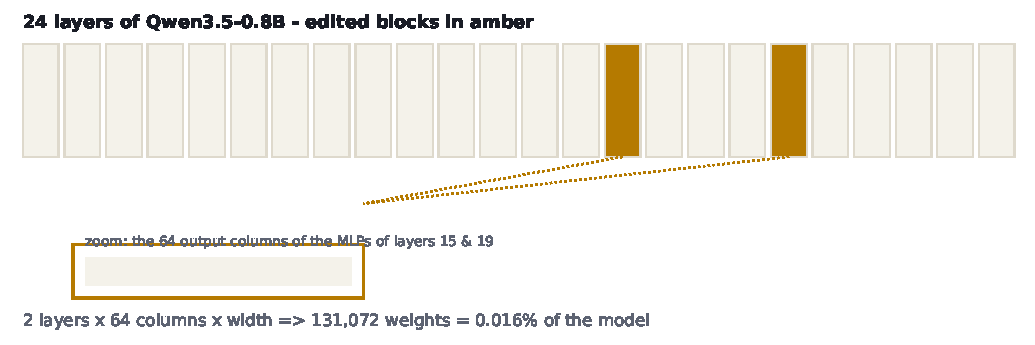
\includegraphics[width=0.98\linewidth]{figures/fig06_edit_anatomy.pdf}
\caption{\bS\; Anatomy of the Exp.~8 edit (block positions \bP, drawing illustrative): two MLP blocks, 64 output columns each.}
\label{fig:anatomyedit}
\end{figure}

\bP\; The negative control is the paper's most reusable idea. The sibling model, Gemma~3~270M, received the same treatment, and its MATH-500 barely moved: 6.8\% at base, then 7.0, 7.6, 7.7, and 7.0\% across 5, 10, 25, and 50 passes. Only 8.5\% of its answers ever hit the token limit, against 93\% for Qwen --- nothing was blocking Gemma, so the edit had nothing to remove. The authors' conclusion: \emph{editing can remove an obstacle that hid an ability; it did not add one}. Figure~\ref{fig:budget} shows both panels, plotted with reported points only, per the discipline of Eq.~\eqref{eq:budgetcurve}.

\begin{equation}\label{eq:budgetcurve}
\mathrm{fidelity}(n), \qquad n \in \{0,\,10,\,25,\,50\}
\end{equation}
with points plotted only at reported budgets --- never interpolated, because a single run per point cannot support a smooth curve.

\begin{figure}[htbp]
\centering
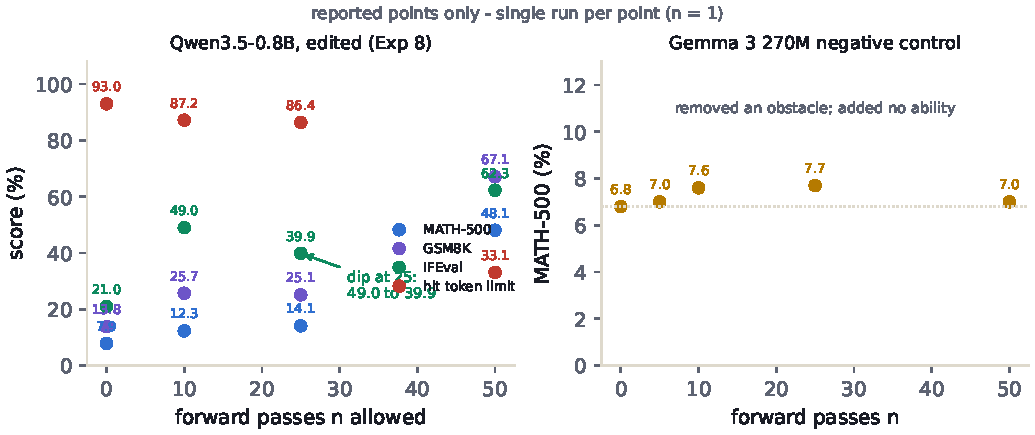
\includegraphics[width=0.98\linewidth]{figures/fig07_budget.pdf}
\caption{\bP\; Left: the four reported Exp.~8 metrics across the feedback budget, including the non-monotonic IFEval dip at 25 passes. Right: the Gemma negative control. One run per point.}
\label{fig:budget}
\end{figure}

\bP\; The replication recipe is unusually cheap for a result of this weight, because the authors released their artefacts: the edited checkpoint is on Hugging Face \cite{wsp-model}, the full logs are in the released repository \cite{wsp-logs}, and a live demo exists \cite{wsp-demo}. The minimal independent check is to evaluate the published edited checkpoint on MATH-500 with thinking mode on and a 32{,}768-token budget, confirming the 48.1/33.1 pair --- then to run the standard direction-ablation baseline on the base model to see what reasoning earned over textbook projection.

Non-monotonicity deserves respect, not smoothing: between 10 and 25 passes, MATH-500 edges up (12.3 to 14.1) while GSM8K sags slightly (25.7 to 25.1) and IFEval drops sharply (49.0 to 39.9), before all three jump at 50 passes. With one seed per point, the only defensible reading is that the edit's effect varies by budget and metric, sometimes sharply --- which is exactly why pre-registered multi-seed budgets are non-negotiable in the benchmark of Section~\ref{sec:lab}.

\bR\; The review grades Exp.~8 the paper's strongest evidence --- measured on three benchmarks, mechanism checked via the token-limit share, negative control included --- while listing the mandatory missing baselines: the standard direction ablation of the same $u$ with no LLM involvement, decoding-time interventions, seeds, and a drift measure on held-out behaviour \cite{maier}.

\section{WRITE: Policies Born from Pure Thought}\label{sec:write}

\bP\; Exp.~5 (MinAtar \cite{minatar}): for each of three games the LLM wrote a $600{\to}32{\to}32{\to}6$ tanh network \emph{starting from all-zero weights} --- no data, no loss, no gradients, no rollouts. Over 1{,}000-episode averages the written policies scored 517.4 (Breakout), 53.1 (Seaquest) and 53.2 (Asterix) against PPO \cite{ppo} baselines trained for 100M and 500M steps (Table~\ref{tab:minatar}). Exp.~6 (Go): a $243{\to}512{\times}6{\to}82$ policy (1{,}480{,}274 parameters) written from zero in a Python sandbox, then allowed 0--50 self-play forward passes. At zero passes it already won the majority of games against two small PPO nets; after 50 passes it beat an \emph{equal-size PPO trained on 20M games}.

\begin{table}[htbp]
\centering
\small
\caption{\bP\; Exp.~5: MinAtar scores, 1{,}000-episode averages.}
\label{tab:minatar}
\begin{tabular*}{\linewidth}{@{\extracolsep{\fill}} l ccc}
\toprule
Game & PPO 100M & PPO 500M & Written, one shot \\
\midrule
Breakout & 15.8 & 25.3 & \textbf{517.4} \\
Seaquest & 5.6 & \textbf{88.9} & 53.1 \\
Asterix & 25.8 & \textbf{55.2} & 53.2 \\
\bottomrule
\end{tabular*}
\end{table}

Reading Table~\ref{tab:minatar} honestly matters: the written policy \emph{crushes} Breakout (about $20\times$ the 500M-step baseline), \emph{loses} to strong PPO on Seaquest, and \emph{nearly ties} on Asterix. The claim the table supports is ``a zero-shot written policy is competitive with heavily trained ones on some games'' --- not a uniform stomp.

\bR\; The Go figures, from the review's reading of the released logs \cite{maier}: against two small PPO nets, 54--55\% at zero passes and 81--84\% at 50; against the equal-size PPO, 26--43\% at zero passes and 70--79\% at 50 (Figure~\ref{fig:go}). The honest headline: with \emph{zero} experience the written policy loses to the strong baseline; with \emph{fifty games} of sandbox refinement it beats it.

\begin{figure}[htbp]
\centering
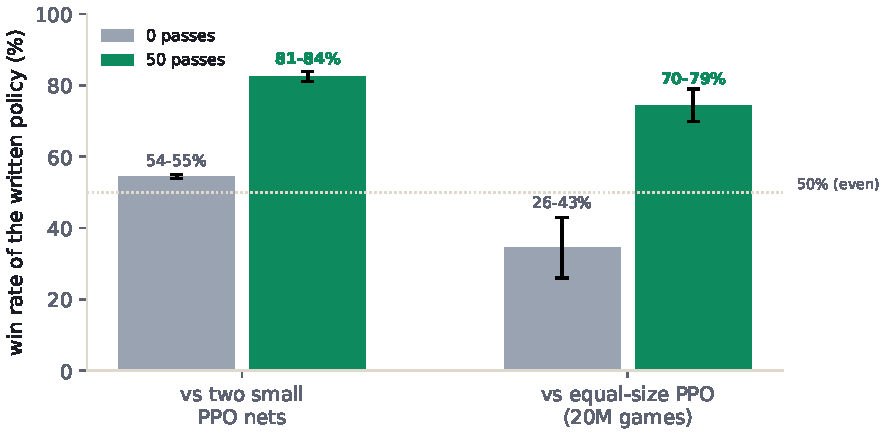
\includegraphics[width=0.68\linewidth]{figures/fig09_go.pdf}
\caption{\bR\; Exp.~6 win rates from the released logs (ranges mid-plotted with error bars); $n=1$ run per condition.}
\label{fig:go}
\end{figure}

Treat the WRITE evidence as two separable claims. \textbf{(W1) Feasibility:} an LLM can produce working weights for structured, well-specified games --- supported strongly by three game policies and the Go result, all beating at least the 100M-step baseline. \textbf{(W2) Generality:} the skill extends to tasks without a public strategy literature --- supported by nothing yet. Almost all popular enthusiasm conflates the two; a reviewer never should. The one experiment that would separate them is procedurally novel, author-blind task families (the WRITE track of Section~\ref{sec:lab}), because a policy transpiled from remembered recipes and a policy genuinely compiled from reasoning differ only on rules nobody has written down.

The mechanisms the post reports split into two families, covered next. One confound deserves a name: MinAtar and Go are \emph{public, well-documented} games, so ``writing from scratch'' may partly be retrieval-plus-transpilation of known strategies. A benchmark with procedurally novel, author-blind rules (Section~\ref{sec:lab}) is the test that separates recall from reasoning.

\section{How Did It Do It? Two Mechanisms}\label{sec:mech}

\bP\; For the written policies, the reported path is \emph{reason $\to$ program $\to$ compile into weights}: state the rules you would follow (a paddle-landing predictor for Breakout; liberty counting and atari detection for Go), then transcribe them into matrix entries. The paddle rule as mathematics,
\begin{equation}\label{eq:compile}
h = \mathrm{ReLU}\bigl(W_1 [b, p]^{\top} + b_1\bigr), \qquad z = W_2 h + b_2,
\end{equation}
with $h_0$ firing when the ball is left of the paddle and $h_1$ when it is right, is exactly Lab~1 (Appendix~D and the shipped \texttt{lab/} folder): seventeen numbers that play passable Breakout. The interesting scientific object is that the LLM performed this transcription across 1.48M parameters \emph{without a compiler} --- the reasoning process is the compiler.

For the math fix, the reported path is \emph{reason $\to$ find a direction $\to$ subtract it} (Eq.~\ref{eq:direction}): diagnose the loop's engine by reading the MLPs of layers 15 and 19, project it out of a few columns, and verify that the token-limit share falls in step with the benchmarks.

\bR\; Two silent-cheat modes deserve explicit attention in any replication. For the compile path: MinAtar and 9$\times$9 Go have enormous public literatures, so a ``written from scratch'' policy may partly transpile remembered strategies; the cheap probe is a set of adversarial positions where textbook heuristics famously fail --- a transpiled textbook fails identically, a genuinely reasoned policy may diverge. For the subtract path: the 50 feedback passes raise the question of what actually got updated between passes --- the direction, the columns, both, or a hand-tuned coefficient. If the passes performed a \emph{search} over candidate directions, the honest label is ``LLM-guided search'', and the correct baseline is the same search with a random initialiser. The released logs are the ground truth for that distinction \cite{wsp-logs}, and reviewers should read them before citing either mechanism as established \cite{maier}.

\bS\; A faithfulness caution that both mechanisms deserve: a reasoning trace is a narrative the model produced, not a read-out of its computation. The traces could be right about the artefact while being generated by processes that never ``represent'' the rule. For WSP that is acceptable --- the claim is about the product, and the product is checkable --- but no one should market the trace as introspective access. The paper's own verification habits (copying-head ground truth; token-limit share; the Gemma control) are the reusable gold: always verify a narrative against a measurement.

\section{Measured vs Anecdote: Sorting the Evidence}\label{sec:judgement}

\bR\; An independent review \cite{maier} sorted every claim by evidence strength, and this document adopts its ordering (Table~\ref{tab:scoreboard}, Figure~\ref{fig:scoreboard}). \textbf{Strong:} the math fix (three benchmarks, a mechanism check via the token-limit share, a negative control); the ramp fix (a measured $0/256 \to 1{,}024/1{,}024$ effect); writing working policies from designed programs (real artefacts beating real baselines). \textbf{Weaker:} the small reading games (four and three correct answers on readable toys); the language identification ($\sim$0.5 confidence among three options); the sycophancy test (three binary picks, a 1-in-8 chance floor, task relaxed before it worked). \textbf{Missing everywhere:} other LLMs, human or automated baselines, repeated runs, cheaper alternatives, and tasks \emph{not} designed by the authors.

\begin{table}[htbp]
\centering
\small
\caption{\bR\; The evidence scoreboard (the review's sort \cite{maier}).}
\label{tab:scoreboard}
\begin{tabularx}{\linewidth}{l >{\raggedright\arraybackslash}X}
\toprule
Strength & What and why \\
\midrule
Strong & Exp.~8: measured on 3 benchmarks; mechanism checked; negative control \\
Strong & Exp.~4: large measured effect, one shot \\
Strong ($n{=}1$) & Exps.~5--6: working policies from a designed program, single runs \\
Weaker & Exps.~1--2: correct but tiny trials, readable layouts \\
Weaker & Exp.~3 language ID: $\approx$0.5 confidence over 3 options (heads match is the solid part) \\
Weaker & Exp.~7: 3 binary picks $=$ 1-in-8 by chance; task relaxed \\
Missing & baselines, seeds, other LLMs, author-blind tasks, cheap alternatives \\
\bottomrule
\end{tabularx}
\end{table}

\begin{figure}[htbp]
\centering
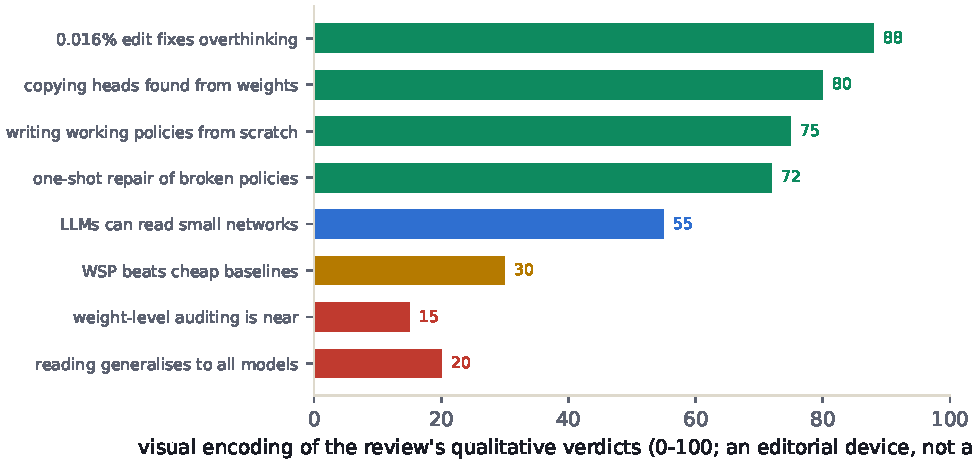
\includegraphics[width=0.9\linewidth]{figures/fig10_scoreboard.pdf}
\caption{\bR\; The scoreboard as thermometers. The heights are my visual encoding of the review's qualitative verdicts --- an editorial device, not a meta-analysis.}
\label{fig:scoreboard}
\end{figure}

The $n{=}1$ problem deserves its own arithmetic. If run-to-run variance can flip a nine-point metric swing (the IFEval dip at 25 passes, Table~\ref{tab:budget}), then \emph{any} single number in the post carries a hidden error bar of at least that size. Three binary classifications succeed by blind luck with probability $2^{-3} = 12.5\%$; language identification at 0.48--0.62 stated confidence sits barely above the 33\% floor of a three-option guess. None of this is damning; all of it demands the same phrase --- \emph{promising, not established} --- and the same remedy: $\geq$5 seeds, pre-registered protocols, and published spread.

The baseline gaps, stated precisely. \textbf{(1)~Decoding control:} would a shorter thinking budget, or a simple stop heuristic, fix the overthinking without touching a single weight? \textbf{(2)~Standard direction ablation:} the same $u$-subtraction with no LLM reasoning anywhere --- the textbook operation of Eq.~\eqref{eq:direction}. \textbf{(3)~Heuristic-code baseline:} the same policies written as ordinary Python; for the WRITE tasks, the honest rival is a human with NumPy in an afternoon. \textbf{(4)~Human-interpreter baseline:} given the same $10{\times}10$ grids, does an interpretability researcher beat the model at Exp.~1? Every one of these is a few GPU-hours or a few hours of expert time. Their absence is the field's to-do list, and it is short --- which is precisely what makes its persistence informative.

\bR\; Two independent signals temper and extend the picture: a deflationary essay argues the case against superhuman framing across all experiments \cite{goedecke}; and a laptop-class replication of a similar weight-reading example with an open 27B model was reported independently on 3~Nov~2026 \cite{willison} --- anecdotal, but hinting the skill is not exclusive to one frontier model. The original authors chose the modest word \emph{sparks}; the evidence matches the word, and the word should survive every retelling.

\section{Small Models, Big Models: Who Benefits?}\label{sec:sizes}

\bS\; The demonstrated frontier divides cleanly by scale. \emph{Small networks} (up to ${\sim}$1.5M parameters) were \textbf{written whole} (MinAtar, Go) and \textbf{repaired} (the ramp actor) --- cases where the entire parameter vector fits within the reasoner's working scope and the task rules are stateable. \emph{Large models} (${\sim}0.8$B) were edited only through \textbf{diagnosis-then-surgery}: the reasoner consumed slices (selected MLP blocks, per-column projections) rather than the whole, and the intervention was a classical closed-form operation guided by reasoning. Writing a large model outright would require holding billions of numbers in context --- nobody claims that yet, and arithmetic says the Go write already strained the format: serialised, 1.48M parameters exceed any context window, so even that write was structured and staged.

\bP\; The experiments also expose the honest boundary of reading: at 270M-class transformers, the \emph{distributed} behaviour (sycophancy) was invisible from weights alone and readable only through activations (Exp.~7), while the \emph{localised} behaviour (the thought loop) yielded to a two-block surgery (Exp.~8). The adjacent literature on probing internal states for behaviour \cite{burns,marks} points the same way: distributed facts can be findable, but not from coordinates alone. A working rule of thumb: \emph{editability} tracks the locality of the misbehaviour, not just the size of the model.

\bS\; The context-window arithmetic, because marketing will wave it away. At roughly two to three characters per serialised number, 1.48M Go parameters approach five million tokens even before overhead --- far beyond any current window --- so even the flagship write cannot have been a raw dump: it was structured, staged, and verified in a sandbox, per the post. The logs repository doubles as the first de-facto weight-interchange protocol; anyone building WSP tooling should study its formats. A productised ``weight clinic'' would chain telemetry $\to$ hypothesis $\to$ targeted read $\to$ intervention $\to$ evaluation, with drift monitoring throughout --- none of it exists off the shelf, all of it is buildable from the released artefacts.

Figure~\ref{fig:blast} puts the two flagship edits on the sparsity meter. Sparsity is necessary-but-not-sufficient evidence of surgical containment: a 0.016\% edit can still shift global behaviour if it hits a hub, which is why the drift measure
\begin{equation}\label{eq:drift}
D = \mathbb{E}_{x \sim \mathcal{P}}\, \mathrm{KL}\bigl(p_\theta(\cdot \mid x) \,\bigl\|\, p_{\theta'}(\cdot \mid x)\bigr)
\end{equation}
belongs in every future report (the post does not give one; WSP-Bench-Lite mandates it).

\begin{figure}[htbp]
\centering
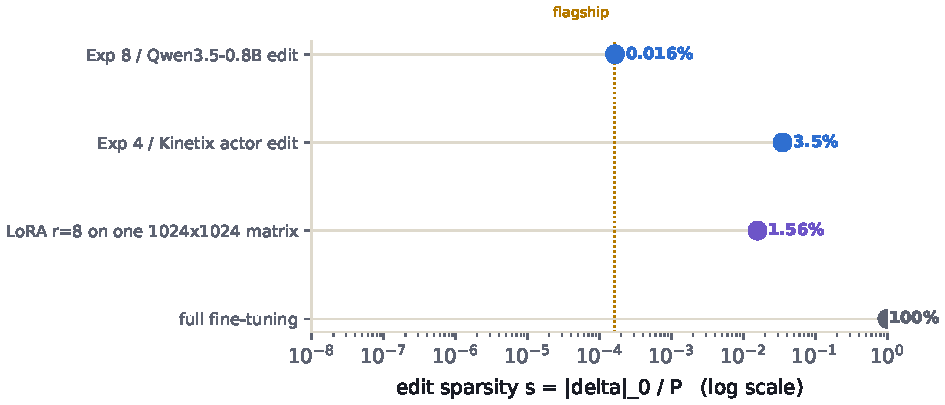
\includegraphics[width=0.85\linewidth]{figures/fig11_blast.pdf}
\caption{\bP\; (Exp values) \bS\; (LoRA and full-FT reference points) The blast-radius meter: edit sparsity $s$ on a log scale.}
\label{fig:blast}
\end{figure}

\begin{table}[htbp]
\centering
\small
\caption{\bS\; What WSP could genuinely help with, by side --- tags follow the review's framing \cite{maier}.}
\label{tab:sizes}
\begin{tabularx}{\linewidth}{l >{\raggedright\arraybackslash}X l}
\toprule
Side & Use & Status \\
\midrule
Small & write/initialise tiny specialist nets & demonstrated (Exps.~5--6) \\
Small & fix broken small policies & demonstrated (Exp.~4) \\
Big & targeted fixes of diagnosed behaviours & demonstrated, one model (Exp.~8) \\
Big & audit/interpret without running & suggested (Exp.~3 heads; Exp.~7 partial) \\
Any & zero-data unlearning, patch ecosystems & speculative (Section~\ref{sec:futures}) \\
\bottomrule
\end{tabularx}
\end{table}

\section{Futures: the Authors' Five Predictions and a Wider Horizon}\label{sec:futures}

\bX\; Everything in this section is speculation --- including the original authors' own five predictions, none tested in the post: (1)~auditing without evaluation (e.g.\ spotting backdoors from weights); (2)~dramatically cheaper optimisation via one-shot initialisation; (3)~zero-data capability steering and unlearning; (4)~recursive self-improvement --- models editing their own or successors' weights; (5)~``true architectural merging'' --- grafting a circuit between different architectures.

\bX\; My extended horizon map (Figure~\ref{fig:horizon}) adds timing and falsifiers. \emph{Now--6 months:} the promised benchmark and harness appear (``currently being built''); replications on other LLMs; first weight-diff patches shared like pull requests. \emph{6--24 months:} signed patch ecosystems (``git for weights''); zero-data unlearning trials; LLM-assisted interpretability as a research tool; one-shot initialisation for edge devices. \emph{2--5 years:} evaluation-free auditing \emph{if} reading generalises; cross-architecture grafting; WSP agents embedded in training pipelines; models programming successors. \emph{5+ years, very speculative:} weights as reviewable source code. Each band carries its falsifier: no benchmark by mid-2027 stalls the near band; replication failures flip the load-bearing ``reading generalises'' switch; direction-ablation baselines matching every fix narrow the unique-value claim to Write.

\bX\; Operationalising the checkable band keeps the map honest: a released benchmark qualifies only if it has $\geq$3 tracks, $\geq$5 seeds, $\geq$2 baselines, and author-blind tasks --- a benchmark without baselines is a demo, and should be recorded as such in any tracking of this band. For ``patch ecosystems'', the gating technology is not machine learning but security engineering: signed weight-diffs with attested origin and licence, plus a diff format compact enough to review by hand (the flagship edit is about a megabyte of floats against a 1.6-gigabyte checkpoint --- three orders of magnitude of reviewability). And discount every horizon by the base rates of adjacent fields: interpretability tools historically take years from paper to production reliability; provenance tooling, two to five.

\begin{figure}[htbp]
\centering
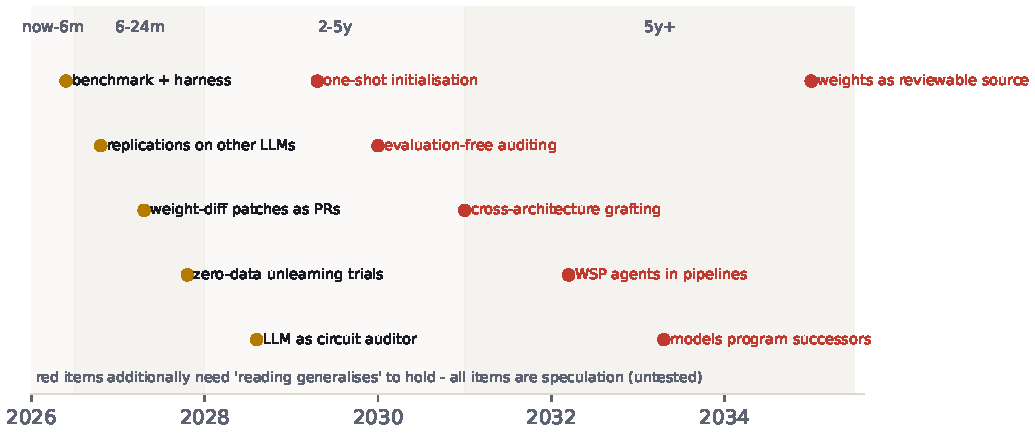
\includegraphics[width=0.98\linewidth]{figures/fig12_horizon.pdf}
\caption{\bX\; The horizon map, 2026--2035. All items are untested predictions; red items additionally require weight-reading to generalise beyond one frontier model.}
\label{fig:horizon}
\end{figure}

\section{The Severe Stuff: a Risk Atlas with Defences}\label{sec:risks}

\bX\; A technique that edits networks by reasoning carries real risks. This section maps them at a \emph{conceptual} level only --- no operational recipes appear anywhere in this document --- and pairs each risk with a defender's toolbox (Table~\ref{tab:risks}, Figure~\ref{fig:risks}). The chapters on defences are the actionable half; the atlas exists so that the defensive work starts \emph{before} it is needed.

\bP\; One risk is anchored in published work rather than speculation: single-direction edits can strip refusal behaviour from open models \cite{refusal}, and the flagship fix is the same operation class --- so ``cheap guardrail-stripping'' is a pre-existing hazard that WSP would only make more accessible. The compute-threshold blind spot follows from the flagship result itself: if a capability can be added by editing 0.016\% of weights with no training run, rules keyed to \emph{training compute} may miss it entirely; capability-based evaluation and post-release change tracking are the obvious correctives. The supply-chain defences borrow directly from adjacent practice: model cards \cite{modelcards}, SBOM-style manifests for weights \cite{sbom}, and the hard lessons of training-data extraction \cite{carlini}.

\begin{table}[htbp]
\centering
\small
\caption{\bX\; The risk atlas: what, and the defence that answers it. Speculative, deliberately non-operational.}
\label{tab:risks}
\begin{tabularx}{\linewidth}{l >{\raggedright\arraybackslash}X}
\toprule
Risk & Defender's toolbox \\
\midrule
Weight-level backdoors & provenance + signed diffs, diff review, weight-space anomaly scans, behavioural red-teaming \\
Safety-training removal & tamper-resistant training, release governance, monitoring derivative checkpoints \\
Compute-threshold blind spot & capability-based evaluation, post-release change tracking \\
Recursive self-improvement & human-in-the-loop sign-off, sandboxed editors, immutable audit logs, self-edit rate limits \\
Licence laundering & weight attestation, watermarking research, model-card diffs \\
Hidden-capability concealment & multiple independent readers, ground-truth probe sets, reader calibration \\
Benchmark gaming & held-out, author-blind tasks (WSP-Bench-Lite's core rule) \\
Over-trust in explanations & verify every narrative against a measurement \\
Power concentration & open replications on small models, public benchmarks \\
What could go right & cheaper customisation, accessible interpretability, safer unlearning --- fund these too \\
\bottomrule
\end{tabularx}
\end{table}

\begin{figure}[htbp]
\centering
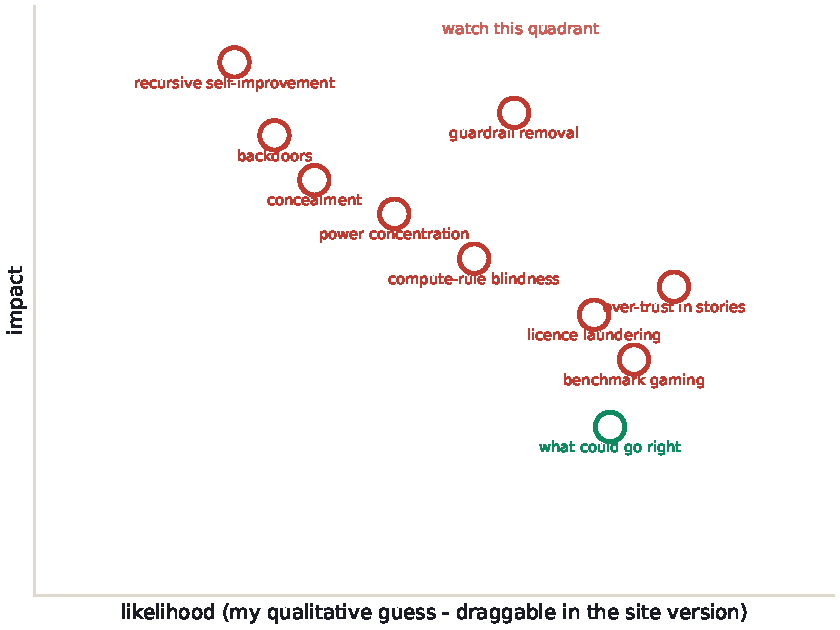
\includegraphics[width=0.6\linewidth]{figures/fig13_risks.pdf}
\caption{\bX\; The risk atlas as a likelihood$\times$impact map (my qualitative placement; the site version is draggable so readers can disagree).}
\label{fig:risks}
\end{figure}

A deployment-grade defence stack, layer by layer. \emph{Provenance:} every published checkpoint carries a signed manifest, and every derivative carries a signed diff against its parent --- the flagship edit is about a megabyte of floats, three orders of magnitude smaller than a checkpoint, which makes diff review genuinely feasible. \emph{Screening:} weight-space anomaly scans plus behavioural red-team suites as continuous integration for models, in the pattern of package scanners. \emph{Governance:} capability-keyed rather than compute-keyed evaluation rules, with mandatory model-card diffs on release. \emph{Epistemics:} no narrative accepted without its measurement, with immutable public audit logs. The detection research gaps are concrete and fundable: whether a 131k-weight edit is statistically detectable without knowing the direction (no published power analysis exists); generalising published tamper-resistant refusal training; attestation formats (a ``weights BOM''); and evaluation protocols that notice capability added without a training run.

On recursive self-improvement, the sober version: compounding requires \emph{reliable evaluation} of one's own edits, and the paper's own budget curves are non-monotonic --- self-editing without trusted external evaluation is more likely to compound error than capability. The dangerous scenario needs a trusted automated evaluator first, which is a monitoring problem, and monitorable. Human sign-off and rate-limited self-edits remain cheap, effective controls while the science catches up.

\section{Het's Lab: Three Runnables and WSP-Bench-Lite}\label{sec:lab}

\bS\; This section is my own contribution, clearly marked. Three labs (all under fifteen lines; verified running on Python~3.12 with NumPy~2.x; each finishes in under a second) make the mechanisms tangible. Lab~1 is the hand-compiled paddle follower of Eq.~\eqref{eq:compile}; Lab~2 performs the direction surgery of Eq.~\eqref{eq:direction} and prints both the exact residual ($\max |u^{\top} W'| \approx 10^{-16}$) and the sparsity/energy trade-off when only the top-$k$ columns are edited (remaining $u$-energy ${\approx}0.74$ at $k{=}8$ of 64); Lab~3 computes the flagship fraction of Eq.~\eqref{eq:sparsity} ($0.0164\%$, which the post rounds to $0.016\%$) and the $2 \times 64 \times 1024$ arithmetic behind 131{,}072, with its [VERIFY] flag preserved. The full sources ship in the package (\texttt{lab/} folder) and in Appendix~D.

\bX\; \textbf{WSP-Bench-Lite} is a community benchmark proposal --- a proposal, with no results yet, because producing results is the community's job. Every rule answers a gap the independent review named (Table~\ref{tab:bench}): three tracks (Read/Fix/Write); tasks authored by non-competing teams and held private between evaluation windows; $\geq$5 seeds per condition; multiple LLM participants; mandatory baselines (decoding tweaks, standard direction ablation, human interpreter, and the same heuristic as ordinary code); metrics that include \emph{edit sparsity} $s$ (Eq.~\ref{eq:sparsity}), \emph{functional drift} $D$ (Eq.~\ref{eq:drift}), the budget-curve fidelity of Eq.~\eqref{eq:budgetcurve}, and cost; pre-registered prompts \cite{prereg}; public logs; and rotating task stewardship in the pattern of capture-the-flag competitions \cite{captureflag}. Reasoning traces are logged for study but never counted as evidence --- only the measured $\Delta$ and its effects score.

\begin{table}[htbp]
\centering
\small
\caption{\bX\; WSP-Bench-Lite: the one-page scoring template (proposal v0.1, Het Patel).}
\label{tab:bench}
\begin{tabularx}{\linewidth}{l l >{\raggedright\arraybackslash}X l}
\toprule
Track & Task type & Mandatory baselines & Metrics \\
\midrule
READ & identify behaviour from weights & human interpreter; same heuristic as code & accuracy, calibration, FPR \\
FIX & repair a seeded defect & decoding tweak; direction ablation; random-direction control & success, sparsity $s$, drift $D$ \\
WRITE & produce a working policy from a spec & random init + short training; best published checkpoint & score, fidelity$(n)$, cost \\
\bottomrule
\end{tabularx}
\end{table}

Implementation notes for harness builders, so the protocol survives contact with reality: targets ship as seeded generators (script plus seed), never as frozen checkpoints, so no participant can overfit one training run; FIX defects are injected by known transformations (sign flips, dead columns, looped directions) so ground truth for ``what changed'' exists; the drift probes are a frozen, task-unrelated set shipped with each task so participants cannot game $D$; every attempt publishes prompt, trace, $\Delta$ coordinates, budget curve, and seeds as JSONL. The whole v0.1 --- thirty tasks across three tracks at $\leq$270M scale --- is a few GPU-weeks; the expensive part is human, recruiting non-competing task authors and holding task sets private between evaluation windows \cite{captureflag}. Governance: rotating stewards, tasks relicensed CC~BY~4.0 after retirement from the live set.

The two results v0.1 should chase first, both informative either way: (1)~does any participant beat the standard direction-ablation baseline on FIX with statistical separation? (If not, the field's flagship demo is an interface to known surgery --- a finding that reframes everything, and is worth having.) (2)~Does WRITE performance survive author-blind, procedurally novel task families? (If not, recall carried the games; if yes, the generality claim graduates to evidence.)

\section{Limitations of This Guide}\label{sec:limitations}

This document inherits the source's limits and adds its own. \bR\; Inherited: every experiment is $n{=}1$; baselines are absent; tasks were author-designed; the primary sources could not all be independently re-opened at build time (fact-check date 5~Nov~2026), so paper-reported figures are transcriptions of the post and its released logs, with every unresolved item listed in Appendix~C. \bS\; Added by me: the qualitative ratings in Tables~\ref{tab:cousins} and \ref{tab:sizes}, the risk placements of Figure~\ref{fig:risks}, the thermometer encoding of Figure~\ref{fig:scoreboard}, and the entire horizon map are editorial devices --- clearly badged --- not measurements. Where my reading of a mechanism could differ from the post's, the text says so (the direction-removal form is explicitly flagged as a teaching approximation). The reader should treat this whitepaper as a carefully sourced secondary work: cite the original post for results, the reviews for verdicts, and this guide only for its teaching apparatus, labs, and benchmark proposal.

\section{Ethics and Responsible Use}\label{sec:ethics}

This guide deliberately contains no operational instructions for harmful edits: the risk atlas names mechanisms at conceptual level only, and every risk is paired with defences. The dual-use asymmetry is acknowledged plainly --- offence in this space is surgical and quiet; defence is infrastructural (signing, scanning, publishing) and, historically, slower. That lag, not any single attack, is the real risk, which is why the defensive research agenda (edit-detection theory, capability-based evaluation standards, attestation formats, reader calibration) is listed in Section~\ref{sec:risks} as fundable, publishable work. On the beneficial side: cheaper customisation for people without data budgets, interpretability that reads like a mechanic's report, unlearning that removes rather than papers over. The honest posture is neither doom nor hype but \emph{defence-first curiosity} --- which is also the practical recommendation of this document.

\section{Conclusion}\label{sec:conclusion}

The claim of weight-space programming is extraordinary in the literal sense: a general-purpose reasoner reading a parameter vector and writing a working fix, with explanations, at a blast radius of 0.016\%. The evidence assembled here supports a precise, modest version of it: \emph{for small-to-mid networks and diagnosed mechanisms, reasoned edits and even whole-network writes reach quality milestones orders of magnitude cheaper than gradient descent} --- with single-run evidence, missing baselines, and honest negative controls. The authors chose the word ``sparks''; the word is load-bearing. What would convert sparks into fire is exactly what Section~\ref{sec:lab} proposes: author-blind tasks, seeds, baselines, drift and sparsity metrics, public logs. Until then, the right stance --- held consistently by this guide's badge system --- is calibrated fascination: read the artefacts, run the labs, demand the measurements, and design the next experiment.

\appendix
\FloatBarrier

\section{Appendix A --- The Fact Sheet}\label{app:factsheet}

\bP\; Structured source data, also shipped as \texttt{research/fact-sheet.json} in the package and served by the companion site at \texttt{/data/fact-sheet.json}. Source: the blog post of 2~Nov~2026 \cite{wsp-post}; model used: GPT-6~Astra; all logs released \cite{wsp-logs}; edited model on Hugging Face \cite{wsp-model}; live demo \cite{wsp-demo}; benchmark and harness ``currently being built''; the post is \textbf{not} peer-reviewed. Fact-check date of this guide: 5~Nov~2026.

\begin{longtable}{@{}c l l >{\raggedright\arraybackslash}p{7.1cm}@{}}
\toprule
\# & Verb & Weights & Reported headline \\
\midrule
\endfirsthead
\toprule
\# & Verb & Weights & Reported headline \\
\midrule
\endhead
\bottomrule
\endfoot
1 & Read & 17{,}253 & Named all 4 games from $10{\times}10$ grids; Breakout at 99\% confidence; no forward passes \\
2 & Read & 23{,}824 & All 3 shapes identified; described outlines while the models draw filled shapes \\
3 & Read & 7.16M & Language 6/6 (confidence 0.48--0.62); copying heads exactly match ground truth: Python 2.1/3.1/3.5, romaji 3.3, English 3.1 \\
4 & Fix & 171{,}664 & One-shot edit of 3.5\% of weights: ramp success $0/256 \to 1{,}024/1{,}024$ \\
5 & Write & $\approx$20{,}486/net$^{a}$ & MinAtar policies from zero: 517.4/53.1/53.2 vs PPO baselines (Table~\ref{tab:minatar}) \\
6 & Write & 1{,}480{,}274 & 9$\times$9 Go from zero: 54--55\% at 0 passes vs small PPO; 70--79\% at 50 passes vs equal-size PPO (Figure~\ref{fig:go}) \\
7 & Read & $\sim$270M$\times$2 & Weights alone 0/4; with attention patterns 3/3; head 10.2: 94.3/0.75 vs 3.5/85.7 \\
8 & Fix & 131{,}072 & Direction subtracted from MLP outputs of layers 15 and 19, 64 columns each: MATH-500 $7.9 \to 48.1$\%, token-limit hits $93 \to 33.1$\% at 50 passes (Table~\ref{tab:budget}); Gemma control flat \\
\end{longtable}

\noindent\small\textsuperscript{a}\,Computed by this guide from the stated architecture, not reported by the authors.

\section{Appendix B --- Glossary (Abridged)}\label{app:glossary}

A 60-term glossary ships with the companion site; the twenty-four most load-bearing terms, one line each. \textbf{$\theta$}: the vector of all parameters. \textbf{Weight space}: the space of all possible $\theta$. \textbf{Parameter count $P$}: how many numbers a model contains. \textbf{Gradient descent}: today's default writer (Eq.~\ref{eq:sgd}). \textbf{Learning rate $\eta$}: the step size of training. \textbf{Forward pass}: one run of the network on an input. \textbf{Receptive field}: the input slice a weight responds to --- why a $10{\times}10$ grid can show a paddle row. \textbf{Permutation symmetry}: hidden units can be relabelled without changing the function --- why naive weight-reading is underdetermined. \textbf{Hypernetwork}: a network trained to output weights \cite{ha}. \textbf{Fast-weight programmer}: a transformer that writes temporary weights as it runs \cite{schlag}. \textbf{Tracr}: a compiler from formal programs to weights \cite{tracr}. \textbf{WSP}: reading, fixing and writing $\theta$ by reasoning (Eq.~\ref{eq:wsp}). \textbf{$\Delta$}: the edit. \textbf{Spec}: the task description conditioning the edit. \textbf{Feedback budget $n$}: forward passes the editor may run. \textbf{Task vector $\tau$}: fine-tuned minus base (Eq.~\ref{eq:taskarith}). \textbf{Induction head}: the two-head copying circuit behind in-context learning (Eq.~\ref{eq:induction}). \textbf{Copying head}: the heads Exp.~3 identified from weights alone. \textbf{Direction removal}: the projection of Eq.~\ref{eq:direction}. \textbf{Edit sparsity $s$}: the blast radius (Eq.~\ref{eq:sparsity}). \textbf{Functional drift $D$}: the containment measure (Eq.~\ref{eq:drift}). \textbf{Token-limit share}: the fraction of answers that ram the generation ceiling --- the mechanism check behind the flagship fix. \textbf{Negative control}: a run designed to show no effect; Gemma's flatness is what validates the flagship claim. \textbf{Author-blind task}: a benchmark task created by someone other than the team being evaluated --- the core rule of WSP-Bench-Lite.

\section{Appendix C --- Open Verification Items}\label{app:verify}

The honesty ledger: everything this guide could not independently confirm at build time (fact-check date 5~Nov~2026). \begin{enumerate}[leftmargin=1.6em, itemsep=1pt]
\item The primary post URL and the two review URLs could not be re-opened at build time; all paper-reported figures are transcriptions from the source fact sheet and the released logs.
\item The hidden size of 1024 behind $131{,}072 = 2 \times 64 \times$ width is inferred by arithmetic, flagged [VERIFY] where used.
\item The weight-space-learning survey identifier (arXiv:2603.10090) is as given in the source post; not independently openable.
\item The Gemma~3 / Qwen3 technical-report identifiers and the Kinetix author list are pending confirmation.
\item The Muon optimizer has an informal citation; to be pinned before this bibliography is cited as final.
\item Three lineage entries (steering, sparse-pruning, delta-debugging) were \emph{dropped} from this document's bibliography pending exact citations; restore them with pinned citations in v1.1.
\item All experiment tables have a single source (the post); the released logs are the cross-check and are cited for that purpose.
\item The MinAtar per-net count 20{,}486 is \emph{computed} by this guide from the stated architecture, not reported by the authors.
\end{enumerate}

\section{Appendix D --- The Three Labs}\label{app:labs}

\bS\; Verified runnable (Python 3.8+, NumPy only). Shipped in \texttt{lab/} with a README.

\begin{lstlisting}[caption={lab/01\_compile\_a\_rule.py --- hand-compile a paddle follower (teaching schematic).}]
import numpy as np
relu = lambda z: np.maximum(z, 0.0)
W1 = np.array([[-1., 1.], [1., -1.]]); b1 = np.array([-0.05, -0.05])   # h0: ball left of paddle, h1: ball right
W2 = np.array([[1., 0.], [0., 0.], [0., 1.]]); b2 = np.array([0., 0.05, 0.])
ACTIONS = ["left", "stay", "right"]
def act(ball, paddle):
    h = relu(W1 @ np.array([ball, paddle]) + b1)
    return ACTIONS[int(np.argmax(W2 @ h + b2))]
assert act(0.2, 0.7) == "left" and act(0.8, 0.3) == "right" and act(0.5, 0.52) == "stay"
\end{lstlisting}

\begin{lstlisting}[caption={lab/02\_direction\_surgery.py --- remove one direction from an MLP output matrix.}]
import numpy as np
rng = np.random.default_rng(0)
d_model, d_ff = 16, 64
W = rng.normal(size=(d_model, d_ff))
u = rng.normal(size=d_model); u /= np.linalg.norm(u)
W_full = W - np.outer(u, u @ W)                       # (I - u u^T) W
print("max |u^T W'| =", np.abs(u @ W_full).max())      # ~ 1e-16
k = 8; cols = np.argsort(-np.abs(u @ W))[:k]            # sparse variant: edit only k columns
W_sp = W.copy(); W_sp[:, cols] -= np.outer(u, u @ W[:, cols])
print(f"edited {k}/{d_ff} columns; remaining u-energy "
      f"{np.linalg.norm(u @ W_sp) / np.linalg.norm(u @ W):.2f}")  # ~0.74
\end{lstlisting}

\begin{lstlisting}[caption={lab/03\_blast\_radius.py --- the sparsity arithmetic of the flagship edit.}]
edited, total = 131_072, 0.8e9
print(f"{edited/total:.4%}")                           # 0.0164%  (paper rounds to 0.016%)
print(2*64*1024)  # 131072 = 2 layers x 64 columns x 1024 (hidden size = inference, VERIFY)
\end{lstlisting}

\section{Appendix E --- Task Schema and Reproducibility Checklist}\label{app:bench}

\bX\; JSON task schema (v0.1), one file per task; the sha256 of the prompt is pre-registered before any run:

\begin{lstlisting}[language={},caption={Task schema, condensed.}]
{ "task_id": "FIX-kine-ramp-01",
  "track": "FIX",
  "author_team": "alpha",        // NEVER the evaluated team
  "target": { "family": "mlp", "shape": [679,128,640,16],
              "init": "ppo_trained", "defect": "seeded: ramp_thruster_sign_flip" },
  "spec": "The car fails the ramp. Fix it.",
  "budget": { "forward_passes": 10, "reasoning_tokens": null },
  "baselines_required": ["random_dir_ablation", "standard_dir_ablation",
                         "decoding_tweak", "human_interpreter"],
  "metrics": ["success_rate", "edit_sparsity_s", "functional_drift_D",
              "budget_curve_fidelity_n", "cost_usd"],
  "seeds": 5,
  "report": { "pre_registered_prompt": "sha256:...", "public_logs": true } }
\end{lstlisting}

Reproducibility checklist for any WSP claim, distilled from this guide's quality gates: \begin{enumerate}[leftmargin=1.6em, itemsep=1pt]
\item Does every number bind to a published table or log?
\item Does every figure carry exactly one evidence badge, and do schematics say so?
\item Are all baselines run --- decoding, standard direction ablation, plain code, human?
\item Are there $\geq$5 seeds, with spread reported and no smooth interpolation between budget points?
\item Is there a negative control, and a mechanism check that ties the narrative to a measurement?
\item Is the edit sparsity $s$ reported, and the functional drift $D$ bounded on held-out behaviour?
\item Were the tasks authored by someone other than the evaluated team?
\item Are the prompt, the reasoning trace, and the $\Delta$ coordinates published?
\end{enumerate}

\bibliography{references}

\end{document}
